\documentclass[twocolumn]{article}

\usepackage[margin=1in]{geometry}

\usepackage{amsmath}
\usepackage{amssymb}
\usepackage{mathtools}

\usepackage{subcaption}

\title{Rendering Depth of Field and Bokeh Using Raytracing}
\author{John Andrews \and Daniel Lubitz}
\date{Spring 2019}

\frenchspacing

\begin{document}
\maketitle

\begin{abstract}
  One hallmark of the modern camera is the distinctive, non-smooth blurring of out-of-focus
  objects, an effect referred to as bokeh, which results from the optical
  properties of the camera's
  system of lenses. This effect is often exploited by photographers for artistic effect,
  but has often been disregarded in graphics due to its complexity and computational cost. Using
  raytracing and a virtual lens system, we simulate this effect.
\end{abstract}

\section{Introduction}
Computer graphics traditionally makes use of a pinhole camera model for
rendering scenes. In this model, each point on the image plane is reached by
exactly one ray of light from the scene, namely the ray defined by the image
plane point and the camera aperture. Consequently, no part of the scene is
blurred or out of focus.

Real photography, however, abandoned pinhole cameras long ago. When they are
constrained by the laws of physics, pinhole cameras are extremely limiting of
the light that reaches the image plane, and therefore require very long exposure
times. Real cameras make use of lens systems to allow more light onto the image
plane, thus reducing exposure times, while maintaining as much as possible of
the tight correspondence between object and image points. They are, however,
inherently limited in the range of points for which they can enforce this
correspondence. For a given position of the image plane, object points that lie
in the corresponding focus plane are projected to a single point, but points not
on that plane project onto a circle, called the \emph{circle of confusion,} that
grows larger as the object point grows more distant from the focus plane. Points
whose circles of confusion are larger than the smallest resolvable disk of the
camera sensor or the human eye appear blurred and out of focus; such points are
outside of the camera's \emph{depth of field.}

Importantly for our discussion, the circle of confusion is not a smooth blur; it
is usually rather sharply defined and more-or-less uniform over its area.
``Bokeh'' refers to this effect; it is the artistic and aesthetic quality of the
out-of-focus parts of an image, in which points of light are blurred into
more-or-less clearly defined shapes.

Bokeh is a very desirable effect to mimic in computer graphics; while defocusing
might be considered the next best thing for real photography, we are now
interested in using it to increase the realism of computer-generated images, and
to allow artists another tool to create different aesthetic effects. It is our
goal to simulate this effect via raytracing.

\section{Related work}
In \cite{McGraw2015}, McGraw simulates defocus blurring by applying synthetic
bokeh as a post-processing effect on an otherwise traditionally-rendered image.
A pure Gaussian convolution modulated by a depth map is a simple approximation
of defocus blurring, though inaccurate; as discussed above,
bokeh consists of sharply defined
shapes, and a Gaussian blur is too dispersed. A more accurate approximation
would be a 2D convolution over the image with a kernel in the shape of the
camera aperture; however, full 2D convolutions are computationally expensive.
McGraw provides a compromise, using multiple separable, 1D linear kernels on
each axis to approximate a sharp 2D convolution kernel, achieving both
perceptual accuracy and speed.

In \cite{Wu2010}, the authors instead use a raytracing approach to accurately
trace the propagation of light through a camera's lens system. They
mathematically model the lens system and refract each ray through each lens
surface before emitting it into the scene. This approach has the advantage of
realistically capturing bokeh and other lens effects such as spherical
aberration, and allows for non-circular aperture shapes and resulting
non-circular bokeh, at the cost of performance; a great many samples per pixel
are required to integrate the light reaching each image point from the lens with
any degree of accuracy. In \cite{Wu2013}, the same team extends this basic
approach with even more sophisticated lens effects, including chromatic aberration.

\cite{JooEtAl2016} go so far as to simulate the lens manufacturing process to
create realistic imperfections and artifacts in their bokeh. Additionally, they
simulate aspheric lenses. Most lenses are composed of spherical surfaces due
to ease of manufacturing, but such lenses suffer from imperfect convergence of
transmitted rays (the above-mentioned spherical aberration). Aspheric lenses can
produce better focus, but are more difficult to model and manufacture. Joo et
al. raytrace such lenses using root-finding methods to produce a very
highly-detailed image of the lens system. However, they do not fully raytrace
the scene; instead, they use the raytraced lens system image to modulate a
traditional rendering, in a manner similar to a 2D convolution.

Our approach is most similar to that of \cite{Wu2010}.

\section{Overview of Gaussian optics}
One of the chief problems of raytracing a lens system is that not all rays cast
towards the first lens surface will actually make it through the system as a whole.
In fact, for any given point on the image plane, only rays from a relatively small
portion of the lens will reach it; the others will be either internally reflected by
some lens element, or fail to clear some internal aperture of the system. Uniformly
sampling the entire lens surface is
therefore very wasteful of resources, and to make the computation reasonably fast,
we require some way to narrow down the sample space. Gaussian optics provides us
with exactly this, in the form of an exit pupil. To that end, we present here an
overview of the relevant concepts from optics. Much of
this material is adapted from \cite{Greivenkamp2004}.

In an optical system, the \emph{aperture stop} is the element that most
restricts the light than can enter the image space of the system. It is
frequently the physically narrowest element, but not always. Any light that
clears the aperture stop will make it to the image plane. The
\emph{exit pupil} is the image of the aperture stop in image space; in effect,
any light that reaches the image plane will come from the direction of a point in
the exit pupil (Figure \ref{fig:pupils}). Hence, the exit pupil defines the sample
space for our raytracing.
Finding the exit pupil requires building up some background machinery.

\begin{figure}
    \centering
    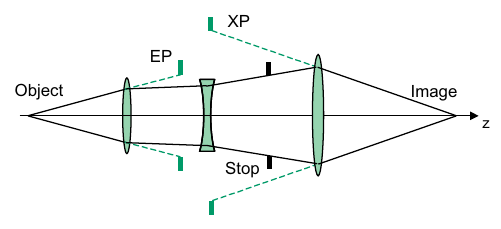
\includegraphics[width=.45\textwidth]{img/pupils.png}
    \caption{The entrance pupil (EP) and exit pupil (XP). The entrance pupil is
    the image of the aperture stop in object space; this would be important were
    we tracing rays from object space into the camera, but for our purposes, we only
    need the exit pupil. Figure from \cite{Greivenkamp2004}.}
    \label{fig:pupils}
\end{figure}

To a first approximation, the properties of an optical system can be determined
using Gaussian optics. This system assumes all surfaces within the system are
ideal refracting or reflecting elements, and makes use of the following
small-angle approximations for the sine, cosine, and tangent functions:
\begin{gather*}
  \sin x \approx \tan x \approx x \\
  \cos x \approx 1
\end{gather*}

These are the first-order Taylor expansions of these functions around 0,
accurate when $|x|$ is small, and are of great usefulness here due to their
linearity.

Gaussian optics considers only systems of spherical elements, axially aligned and
rotationally symmetric about that axis. By convention, the optical axis of the
system is assumed to be the $z$ axis,
with object space towards negative $z$ and image space towards positive $z$. Each surface
is modeled as a single plane perpendicular to the optical axis at the surface's \emph{vertex},
the point at which it intersects the axis. The radius of curvature of the surface is a
signed quantity indicating the concavity of the surface; specifically, it is the
directed distance from the surface vertex to its center of curvature. Hence, a negative
radius of curvature indicates that the surface is concave towards object space, and a
positive radius of curvature indicates that it is convex towards the same.

The basic technique of Gaussian optics is to reduce systems of many surfaces to a single
set of points on the optical axis, the \emph{cardinal points,} (and their corresponding
planes perpendicular to the axis): the front and rear \emph{focal points,} and the front and rear \emph{principal points}. Once these are known, the image of any object point can be found
via similar triangle analysis using the following
principle: any ray through the front focal point that intersects the front principal plane
at a height $h$ from the optical axis emerges from the rear principal plane at the same
height parallel to the axis, and vice versa (Figure \ref{fig:surface_cardinal_points}).

\begin{figure}[ht]
    \centering
    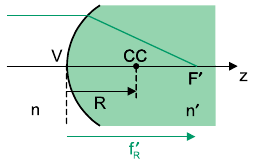
\includegraphics[width=.45\textwidth]{img/surface_cardinal_points.png}
    \caption{The rear cardinal points of a single surface. The principal
    points are coincident with the surface vertex $V$. As demonstrated by the red
    ray, any object-space ray incident on the front principal plane is transmitted
    as a ray through the rear focal point $F'$; a similar rule holds for image space
    rays and the front focal point $F$. $CC$ is the center of curvature. Figure from
    \cite{Greivenkamp2004}.}
    \label{fig:surface_cardinal_points}
\end{figure}

For a single surface, the principal planes are coincident at the surface's vertex.
The focal points are found as follows:
\begin{gather*}
    \text{Optical power } \Phi = \frac{n' - n}{R} \\
    \text{Effective focal length } f_E = \frac{1}{\Phi} \\
    \text{Front focal distance } f_F = -nf_E \\
    \text{Rear focal distance } f'_R = n'f_E
\end{gather*}
where $n$ and $n'$ are the indices of refraction on, respectively, the object space
side and the image space side of the surface, and $R$ is the radius of curvature. The
focal distances are the signed
distances from the surface vertex to the corresponding focal points (Figure
\ref{fig:surface_cardinal_points}).

For two elements enclosing a material with index of refraction $n_2$, with indices
$n = n_1$ on the object space side and $n' = n_3$ on the image space side of the pair,
we can find their joint principal planes via the following:
\begin{gather*}
    \tau = \frac{t}{n_2} \\
    \Phi = \Phi_1 + \Phi_2 - \Phi_1\Phi_2\tau \\
    \frac{d}{n} = \frac{\Phi_2}{\Phi}\tau \\
    \frac{d'}{n'} = -\frac{\Phi_1}{\Phi}\tau
\end{gather*}
In the above, $t$ is the signed distance from the first element's rear principal
plane to the second element's front principal plane; $\Phi_1$ and $\Phi_2$ are the
optical powers of the first and second elements respectively, and $\Phi$ is the
joint optical power; $d$ is the signed distance from the first element's front
principal plane to the joint front principal plane; and $d'$ is the signed distance
from the second element's rear principal plane to the joint rear principal plane
(Figure \ref{fig:gaussian_reduction}).
The joint focal points can be found as above for a single surface, with the exception
that $f_F$ and $f'_R$ are now signed distances from the front and rear principal planes
respectively, rather than from a surface vertex. Systems of more than two elements
can be reduced by repeatedly applying this procedure to adjacent pairs of elements.

\begin{figure}[ht]
    \centering
    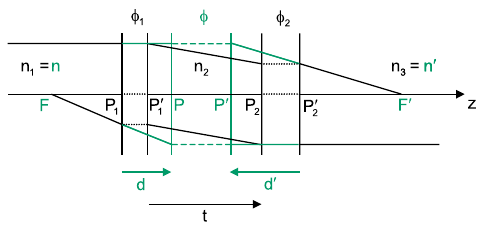
\includegraphics[width=.45\textwidth]{img/gaussian_reduction.png}
    \caption{Gaussian reduction of a two-element system. Figure from
    \cite{Greivenkamp2004}.}
    \label{fig:gaussian_reduction}
\end{figure}

To determine which lens element acts as the system aperture stop, we perform a
\emph{paraxial raytrace} through the system. This is a trace of a ray very near the
optical axis, which remains near the optical axis throughout the system, and
makes use of the small-angle approximations described earlier. The procedure
involves alternating two equations: the transfer equation to determine the
new height of the ray as it arrives at the next element's front principal plane,
and the refraction equation to determine the new angle of the ray as it exits
the element's rear principal plane:
\begin{gather*}
    \text{Refraction: } n'u' = nu - y\Phi \\
    \text{Transfer: } y' = y + u't'
\end{gather*}

In the above, $u$ is the angle of the ray incident on an element's front principal
plane, and $u'$ is the angle of the ray exiting the element's rear principal plane;
$n$ and $n'$ are the object and image space indices of refraction around the element;
$y$ is the (signed) height above the optical axis of the ray's intersection with the
element's principal planes, and $y'$ is the height of the intersection with the
next element's principal planes; $t'$ is the signed distance from the element's rear
principal plane to the next element's front principal plane; and $\Phi$ is the
element's optical power (Figure \ref{fig:paraxial_raytrace}).

\begin{figure}[ht]
    \centering
    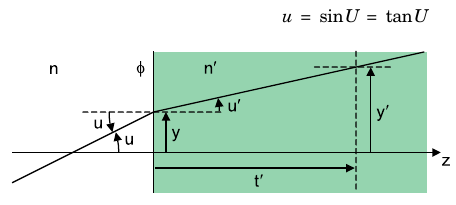
\includegraphics[width=.45\textwidth]{img/paraxial_raytrace.png}
    \caption{Paraxial raytracing. Figure from \cite{Greivenkamp2004}.}
    \label{fig:paraxial_raytrace}
\end{figure}

The refraction equation is based on Snell's law of refraction, using the small-angle
approximation. The full law is this:
\begin{equation*}
    n\sin\theta = n'\sin\theta'
\end{equation*}

The $-y\Phi$ term in the paraxial refraction equation accounts for the changing
surface normal as distance from the axis increases.

During a paraxial raytrace, we can record the ratio $|y| / a$ for each element
of the system, where $a$ is the aperture radius of that element. The element for
which this ratio is greatest --- the element for which the ray passes proportionally
closest to the aperture --- is the system aperture stop. Once we know which element
is the system aperture stop, we can reduce the portion of the system behind that
element and perform similar triangle analysis to find its image in the image space
of the system; that image, finally, is the exit pupil.

This procedure consists of a great many steps, but each one individually is very
simple. Computationally, this calculation is among the least expensive parts of
our algorithm.

\section{Modeling the lens system}
Our model considers only spherical optical surfaces. We specify the lens system
in its own coordinate space in units of millimeters, axially aligned on the $z$
axis with object space towards negative $z$, the convention of Gaussian optics.
Surfaces are listed from object space to image space, with
each surface specified by its radius of curvature, the diameter of its
aperture, the index of refraction of the material on the image space side of
the surface, and the distance to the next surface's vertex. A surface with a
radius of $0.00$ is assumed to be planar, and the medium in front of the system
is assumed to be air, with index of refraction $1.00$. A diaphragm in the system
is modeled as a planar surface with air on either side of it. Figure \ref{fig:lens}
shows one lens configuration using this representation. It should be noted
that this is the same representation used by \cite{Wu2010}, and
we used the lens system configurations presented in that paper for our examples.

\begin{figure}[h]
    \centering
    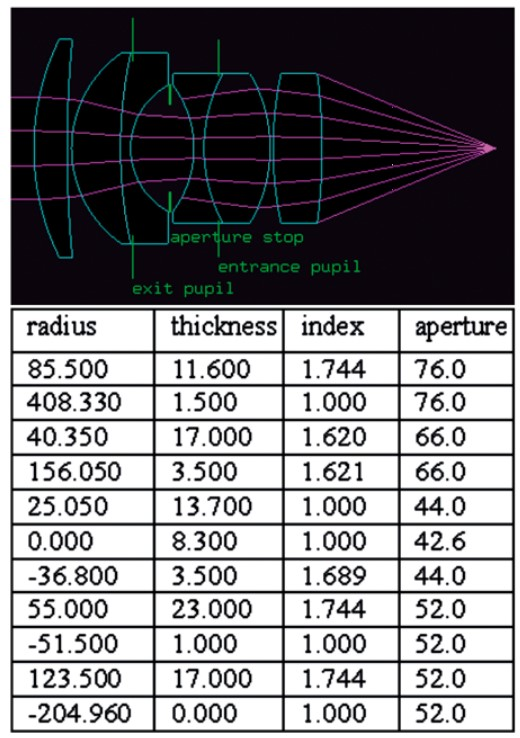
\includegraphics[scale=0.4]{img/lens.jpg}
    \caption{The particular measurement for the lens assembly used for our
    renderings. Figure from \cite{Wu2010}.}
    \label{fig:lens}
\end{figure}

After loading the lens system measurements, our implementation performs a
paraxial raytrace, as described above, to determine which element of the system
acts as the system aperture stop. We then perform a Gaussian reduction on the
portion of the system behind the aperture stop, closer to image space, and use
that reduction to find the location and radius of the exit pupil, and this
concludes our preprocessing of the lens system.

During raytracing, the lens system can be queried for a ray through any point in
the image. To generate a ray, we select a uniformly random point in the exit
pupil and create a ray from the queried image point through the pupil point,
which we then trace through the lens system.

Due to the way we model the lens system, there is no need to test the ray for
intersection with every surface for every step of the lens system trace, or to add
an epsilon to intersection points to overcome floating-point error; we know
exactly the order in which each ray will intersect the surfaces, and we simply
ignore all others for each step. So, in optical order,
we intersect the ray with the sphere (or plane) of the next lens surface and
determine the surface normal at the intersection point. We use Snell's law to
compute the refraction direction, and use this to create a new ray for the next step
of the trace.

While the calculation of the exit pupil provides very useful boundaries on our sample
space, it is calculated via Gaussian optics, which is an approximation;
sampling the exit pupil greatly increases the probability that any given ray will
make it through the lens system, but does not provide a guarantee. Therefore, at
each surface, we compare the intersection point's distance from
the $z$ axis with the aperture radius of that surface, and discard the ray if it
exceeds that radius.

After the last surface has been intersected, we transform the final ray into scene
space using the inverse of the camera view matrix. From there, the color
corresponding to this ray is determined via traditional recursive raytracing.
For a single pixel, we cast many rays through the lens, and determine the final
color by simple average of the colors returned by those rays.

\section{Other implementation details}
Our implementation makes use of KD-trees to accelerate raytracing on triangle
meshes. After loading the geometry data for each mesh, we compute the centroids
of each triangle, and sort them along each axis. Using this, we construct the
KD-tree for the mesh by recursively subdividing the mesh's bounding box at the
median along the axis with the greatest range of centroids.
Triangles that span the divide are included in both subtrees. When testing a ray
for intersection with a mesh, we first recursively test for intersection with
the KD-tree bounding boxes to generate a list of potentially intersected faces.

We also implemented vertex normal interpolation on the CPU for triangular
faces, to allow triangle meshes to appear smooth in our raytraced images. Once
an intersection point has been determined on a triangle, we can compute the
barycentric coordinates $\alpha, \beta, \gamma$ of that point using Cramer's
rule. Then, we compute the internal surface normal $\tilde{n}$ as follows:
\begin{gather*}
  n = \alpha\tilde{n}_a + \beta\tilde{n}_b + \gamma\tilde{n}_c \\
  \tilde{n} = \frac{n}{\|n\|}
\end{gather*}
where $\tilde{n}_a, \tilde{n}_b, \tilde{n}_c$ are the unit vertex normals of the
vertices corresponding to $\alpha, \beta$, and $\gamma$ respectively.

Our implementation utilizes multithreading to accelerate overall rendering times.
Upon starting a rendering, we divide the image into a grid of (approximately)
$20\times 20$ pixel patches and spawn as many threads as the system has physical
processors. Each thread renders a single patch at a time, querying the main
image structure for the next unassigned patch after finishing each patch.
Raytracing is an inherently parallel algorithm; each pixel in the image can be
computed independently of any other pixel. Hence, we see significant speedup using
this scheme.

\section{Early results and challenges}
We began development by implementing a single thin lens and placing it in the world.
This proof of concept allowed us to ensure that we could produce a coherent image
from a simple system. One feature of this early test platform was that we could
trace rays from a point on the image plane to the entire surface of the lens, then
visualize those rays. This enabled us to see whether or not the lens was refracting
the rays correctly.

\begin{figure}[h]
    \centering
    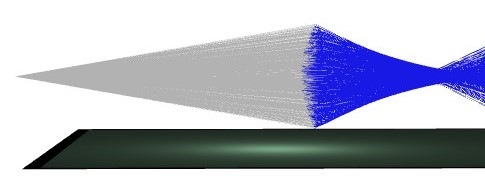
\includegraphics[scale=0.45]{img/lotsa_rays.jpg}
    \caption{Visualization of one pixel sampling the entire lens surface in the test
    environment. Because of the spherical lens, the rays do not converge to a single
    point.}
    \label{fig:lotsa_rays}
\end{figure}

We were able to faintly capture the circle of confusion, meaning our approach was working.
The trouble was getting an image that was meaningful, as we were not using proper measurements
at this point and the positioning  and size of the image plane, lens, and object were
essential guesswork.

\begin{figure}[h]
    \centering
    
\includegraphics[scale=1.0]{img/ghost_coc.jpg}
    \caption{The circle of confusion created by a small sphere in front of a single thin
    lens.}
    \label{fig:ghost_coc}
\end{figure}

\begin{figure}[h]
    \centering
    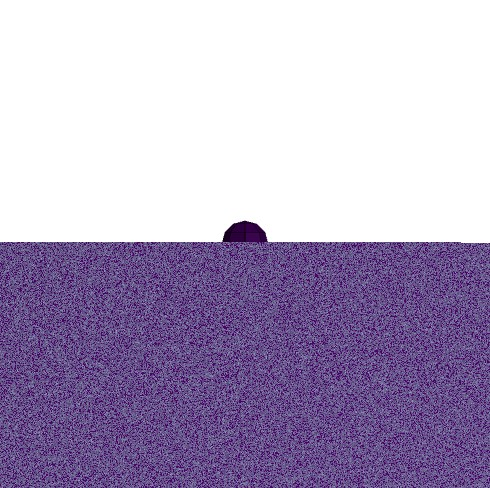
\includegraphics[scale=0.5]{img/static.jpg}
    \caption{A half-raytraced image of a sphere in front of a thin lens. Due to lack of
    measurements, the sphere was not the correct size nor in the correct position to get
    an image from. Some rays missed the sphere and some hit it, creating the static pattern
    seen here. This is also an example of what may happen with a low smaple count.}
    \label{fig:static}
\end{figure}

The implementation of the thin lens was different from the final project due to this
lens being an actual object the exists in the scene. It was made using two intersecting
spheres of the same diameter. A hit from a ray on one sphere was checked to make sure
it was inside the other in order to be considered on the lens surface.

The transition to raytracing the full lens assembly was where
the most bugs arose, particularly sign errors and vector math. In order to send a ray
fully through the assembly, we needed a system that would perform refraction from an
arbitrary material into an arbitrary material at a point where the normal may be facing
forwards or backwards. It also needed to check for conditions such as collision with
one of the stops or a ray refracting at such a steep angle that it would not collide
with the next lens. This complexity required many attempts in order to nail down the
math.

\begin{figure}
    \centering    
    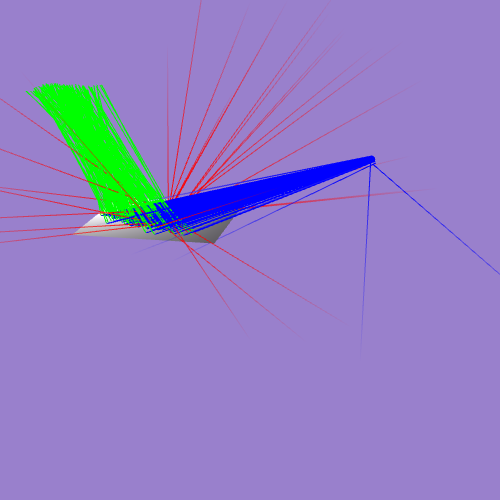
\includegraphics[width=.4\textwidth]{img/backwards_rays.png}
    \caption{An early bug from our lens assembly implementation. Here we see the
    effects of a single sign error in our refraction logic, which prevented the
    emerging rays from converging and caused an occasional ray to actually be
    emitted backwards from the camera.}
    \label{fig:backwards_rays}
\end{figure}

The nature of raytracing is heavy computation. Because of the way our system
gathers light for each pixel from all possible directions out of the lens, we need
a large number of samples to generate a realistic image. This hurt testing as we were
unable to quickly check if a change to an algorithm actually fixed anything. Adding
multithreading dramatically increased our ability to produce images and test at an
acceptable rate.

\section{Results and discussion}
All of the results we present here were rendered on a Lenovo Thinkpad T450s laptop
with an Intel i7 4-core processor. We are able to produce accurate images that exhibit
the desired depth of field and bokeh effects at $200\times200$ pixels, with 250 lens
samples per pixel, in under ten minutes.

All of our results used the lens assembly pictured in Figure \ref{fig:lens}, which has
an approximate effective focal length of 100 mm. Different depths of field and bokeh
qualities may be achieved by different lens configurations; this is one possible avenue
for future work.

\begin{figure}
    \centering
    \begin{subfigure}[b]{.3\textwidth}
        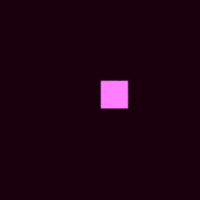
\includegraphics[width=\textwidth]{img/magenta_square_1_correct.png}
    \end{subfigure} \\
    \begin{subfigure}[b]{.3\textwidth}
        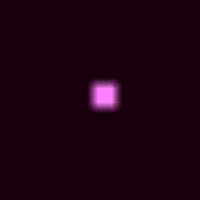
\includegraphics[width=\textwidth]{img/magenta_square_2_correct.png}
    \end{subfigure} \\
    \begin{subfigure}[b]{.3\textwidth}
        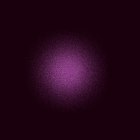
\includegraphics[width=\textwidth]{img/magenta_square_3.png}
    \end{subfigure}
    \caption{A progression of images of a single square light source as the
    camera zooms further out and the light becomes more out of focus. Note that
    the defocus blur is remarkably smooth; this may be a result of the specific lens
    configuration used. Other combinations of focal lengths and aperture diameters
    will produce different bokeh qualities.}
    \label{fig:magenta_square}
\end{figure}

\begin{figure}[h]
    \centering
    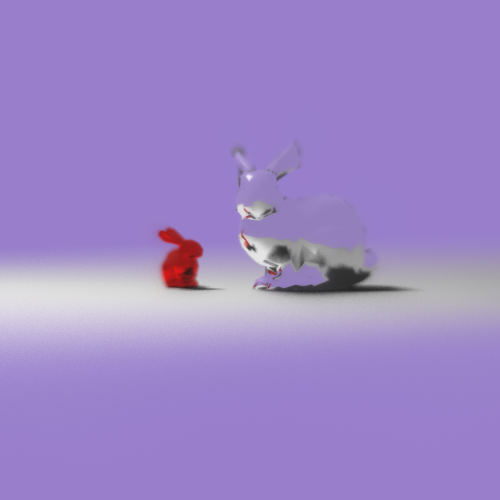
\includegraphics[scale=0.45]{img/hires_blurry_buns.png}
    \caption{High resolution render of reflective bunnies. Depth of field is clearly
    apparent with the ground plane. $500\times 500$ pixels,
    500 lens samples per pixel, approximately 2.5 hours.}
    \label{fig:hires_blurry_buns}
\end{figure}

\begin{figure}[ht]
    \centering
    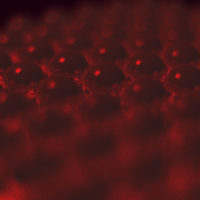
\includegraphics{img/red_sphere_array_correct.png}
    \caption{An array of red reflective spheres under a red light, with noticeable
    bokeh in the out-of-focus specular highlights. $200\times 200$ pixels, 250 lens
    samples per pixel, roughly 8:15 minutes.}
    \label{fig:red_sphere_array_correct}
\end{figure}

\begin{figure}[h]
    \centering
    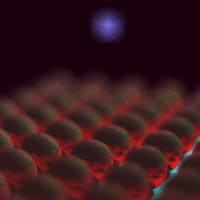
\includegraphics[scale=1.0]{img/red_sphere_array_lights_correct.png}
    \caption{Array of red reflective spheres with blue light patch showing circular
    bokeh effect. The blurring on the light is significantly smoother than we
    would like; c.f. the discussion under Figure \ref{fig:magenta_square}.
    $200\times 200$ pixels, 250 lens samples per pixel, approximately 9 minutes.}
    \label{fig:red_sphere_array_lights_correct}
\end{figure}

\section{Future work}
All lenses and other elements in the lens assembly are perfectly spherical or circular.
One possible avenue for further study would be to implement the option to change these
parameters and introduce aspheric lenses to the system. Additionally, rendering an
image using a non-circular aperture stop would yield particularly interesting results,
given that the circle of confusion's shape on the image plane is dictated by the shape
of the aperture stop. This would involve more sophisticated raytracing algorithms as
the intersection detections would no longer be simple equations. Actual modeling of the
lens surfaces could be done, but that would increase computation time significantly.
Pupil calculation would also need to be reworked if the aperture could change shape.

In our system, we model light as a single color: white. In reality, light is not a simple
white but is instead made up of different wavelengths. In order to accurately model lens
interactions with varying wavelengths of light, a more complete version of Snell's law
would need to be put in place. In addition, finding a way to make raytracing with multiple
rays each with individual wavelengths efficient is non-trivial. Having more than one color
of ray to cast means many times more rays in total to compute. Adding this would allow
the system to create chromatic aberration artifacts, adding to the realism of the image.

Taking the idea of replicating camera effects further, another feature to implement could
be lens flare. This results from scattering in the lens assembly, usually caused by
imperfections in the material makeup of the lens elements. Another artifact not modelled is
refection of light off of the lenses. We only perform complete refraction but some of the
light is reflected internally.

Because our system is modular in the sense that the lens assembly is specified through a
file separate from the rest of the scene, it would be possible to experiment with various
types of configurations, including setups that feature mirrors. In this way, perhaps
certain reflecting telescopes and microscopes could even be modeled.

The major performance bottleneck of our system is not the lens assembly itself, but
rather the recursive raytracing that takes place in the scene. This is especially
expensive when rendering high-complexity meshes like the Stanford Bunny. Nonetheless,
since each trace of the lens assembly is essentially the same, it would be
possible, and possibly beneficial, to calculate the lens samples offline and store
them as part of the lens configuration. This would require a large amount of storage;
each pixel in the image has a different set of samples. It is unclear if this would
result in a speed increase during the actual rendering, and this might be an interesting
experiment.

A possible enhancement to the efficiency of the raytracer would be to use a dynamic
sampling technique. Because we are required to use many a large number of rays for
each pixel, being able to cut down on that requirement would mean great time savings.
For this technique, we would only send out for pixels where there is a large variation
in returned color. The greater the variation, the more samples would be necessary to
capture the true result. For pixels where most of the rays come back looking the same,
not many more rays would need to be used to approximate the true color.

\section{Attributions}
\paragraph{John Andrews}
Wrote the raytracing engine, KD-tree implementation, and vertex normal interpolation.
Wrote parsers for scene and materials files. Did the optics math for finding
the exit pupil. Integrated the lens and lens assembly data structures with the rest
of the raytracer. Rendered most of the examples.

\paragraph{Daniel Lubitz}
Created early test environment to ensure viability of strategies,
worked out initial lens refraction math,
implemented early version of raytracing system for lenses,
developed lens and lens assembly data structures and file conventions,
Windows compatibility debugging.

%\clearpage
\bibliographystyle{apalike}
\bibliography{bibliography}

\end{document}
